%
% Main document
% ===========================================================================
% This is part of the document "Project documentation template".
% Authors: brd3, kaa1
%

%---------------------------------------------------------------------------
\documentclass[
	a4paper,					% paper format
	10pt,							% fontsize
	twoside,					% double-sided
	openright,				% begin new chapter on right side
	notitlepage,			% use no standard title page
	parskip=half,			% set paragraph skip to half of a line
]{scrreprt}					% KOMA-script report
%---------------------------------------------------------------------------

\raggedbottom
\KOMAoptions{cleardoublepage=plain}			% Add header and footer on blank pages


% Load Standard Packages:
%---------------------------------------------------------------------------
\usepackage[standard-baselineskips]{cmbright}

\usepackage[ngerman,english]{babel}										% english hyphenation
%\usepackage[latin1]{inputenc}  							% Unix/Linux - load extended character set (ISO 8859-1)
\usepackage[ansinew]{inputenc}  							% Windows - load extended character set (ISO 8859-1)
\usepackage[T1]{fontenc}											
\usepackage{textcomp}													% additional symbols
\usepackage{ae}																% better resolution of Type1-Fonts 
\usepackage{fancyhdr}													% simple manipulation of header and footer 
\usepackage{etoolbox}													% color manipulation of header and footer
\usepackage{graphicx}                      		% integration of images
\usepackage{float}														% floating objects
\usepackage{caption}													% for captions of figures and tables
\usepackage{booktabs}													% package for nicer tables
\usepackage{tocvsec2}													% provides means of controlling the sectional numbering
%---------------------------------------------------------------------------

% Load Math Packages
%---------------------------------------------------------------------------
\usepackage{amsmath}                    	   	% various features to facilitate writing math formulas
\usepackage{amsthm}                       	 	% enhanced version of latex's newtheorem
\usepackage{amsfonts}                      		% set of miscellaneous TeX fonts that augment the standard CM
\usepackage{amssymb}													% mathematical special characters
\usepackage{exscale}													% mathematical size corresponds to textsize
%---------------------------------------------------------------------------

% Package to facilitate placement of boxes at absolute positions
%---------------------------------------------------------------------------
\usepackage[absolute]{textpos}
\setlength{\TPHorizModule}{1mm}
\setlength{\TPVertModule}{1mm}
%---------------------------------------------------------------------------					
			
% Definition of Colors
%---------------------------------------------------------------------------
\RequirePackage{color}                          % Color (not xcolor!)
\definecolor{linkblue}{rgb}{0,0,0.8}            % Standard
\definecolor{darkblue}{rgb}{0,0.08,0.45}        % Dark blue
\definecolor{bfhgrey}{rgb}{0.41,0.49,0.57}      % BFH grey
%\definecolor{linkcolor}{rgb}{0,0,0.8}     			% Blue for the web- and cd-version!
\definecolor{linkcolor}{rgb}{0,0,0}        			% Black for the print-version!
%---------------------------------------------------------------------------

% Hyperref Package (Create links in a pdf)
%---------------------------------------------------------------------------
\usepackage[
	pdftex,ngerman,bookmarks,plainpages=false,pdfpagelabels,
	backref = {false},										% No index backreference
	colorlinks = {true},                  % Color links in a PDF
	hypertexnames = {true},               % no failures "same page(i)"
	bookmarksopen = {true},               % opens the bar on the left side
	bookmarksopenlevel = {0},             % depth of opened bookmarks
	pdftitle = {Template for Bachelor Thesis},	   	% PDF-property
	pdfauthor = {brd3},        					  % PDF-property
	pdfsubject = {LaTeX Template},        % PDF-property
	linkcolor = {linkcolor},              % Color of Links
	citecolor = {linkcolor},              % Color of Cite-Links
	urlcolor = {linkcolor},               % Color of URLs
]{hyperref}
%---------------------------------------------------------------------------

% Set up page dimension
%---------------------------------------------------------------------------
\usepackage{geometry}
\geometry{
	a4paper,
	left=28mm,
	right=15mm,
	top=30mm,
	headheight=20mm,
	headsep=10mm,
	textheight=242mm,
	footskip=15mm
}
%---------------------------------------------------------------------------

% Makeindex Package
%---------------------------------------------------------------------------
\usepackage{makeidx}                         		% To produce index
\makeindex                                    	% Index-Initialisation
%---------------------------------------------------------------------------

% Glossary Package
%---------------------------------------------------------------------------
% the glossaries package uses makeindex
% if you use TeXnicCenter do the following steps:
%  - Goto "Ausgabeprofile definieren" (ctrl + F7)
%  - Select the profile "LaTeX => PDF"
%  - Add in register "Nachbearbeitung" a new "Postprozessoren" point named Glossar
%  - Select makeindex.exe in the field "Anwendung" ( ..\MiKTeX x.x\miktex\bin\makeindex.exe )
%  - Add this [ -s "%tm.ist" -t "%tm.glg" -o "%tm.gls" "%tm.glo" ] in the field "Argumente"
%
% for futher informations go to http://ewus.de/tipp-1029.html
%---------------------------------------------------------------------------
\usepackage[nonumberlist]{glossaries}
\makeglossaries

\newglossaryentry{BibTeX}{name={BibTeX},description={Program for the creation of 	bibliographical references and directories in \TeX or \LaTeX documents}}
\newglossaryentry{Index}{name={Index},description={Index with keywords from text}}



%---------------------------------------------------------------------------

% Intro:
%---------------------------------------------------------------------------
\begin{document}                              	% Start Document
\settocdepth{section}														% Set depth of toc
\pagenumbering{roman}														
%---------------------------------------------------------------------------

\providecommand{\heading}{Data Collection and Preparation for Currency Adaptation}		%  Insert Title of Thesis here					% Titel der Arbeit aus Datei titel.tex lesen
\providecommand{\versionnumber}{0.1}			%  Hier die aktuelle Versionsnummer eingeben
\providecommand{\versiondate}{17.04.2021}		%  Hier das Datum der aktuellen Version eingeben				% Versionsnummer und -datum aus Datei version.tex lesen

% Set up header and footer
%---------------------------------------------------------------------------
\makeatletter
\patchcmd{\@fancyhead}{\rlap}{\color{bfhgrey}\rlap}{}{}		% new color of header
\patchcmd{\@fancyfoot}{\rlap}{\color{bfhgrey}\rlap}{}{}		% new color of footer
\makeatother

\fancyhf{}																		% clean all fields
\fancypagestyle{plain}{												% new definition of plain style	
	\fancyfoot[OR,EL]{\footnotesize \thepage} 	% footer right part --> page number
	\fancyfoot[OL,ER]{\footnotesize \heading, Version \versionnumber, \versiondate}	% footer even page left part 
}

\renewcommand{\chaptermark}[1]{\markboth{\thechapter.  #1}{}}
\renewcommand{\headrulewidth}{0pt}				% no header stripline
\renewcommand{\footrulewidth}{0pt} 				% no bottom stripline

\pagestyle{plain}
%---------------------------------------------------------------------------


% Title Page and Abstract
%---------------------------------------------------------------------------
%%
% Project documentation template
% ===========================================================================
% This is part of the document "Project documentation template".
% Authors: brd3, kaa1
%

\begin{titlepage}


% BFH-Logo absolute placed at (28,12) on A4 and picture (16:9 or 15cm x 8.5cm)
% Actually not a realy satisfactory solution but working.
%---------------------------------------------------------------------------
\setlength{\unitlength}{1mm}
\begin{textblock}{20}[0,0](28,12)
	
\includegraphics[scale=1.0]{images/BFH_Logo_B.png}
\end{textblock}

% Institution / titel / subtitel / authors / experts:
%---------------------------------------------------------------------------
\begin{flushleft}

\vspace*{21mm}

\fontsize{26pt}{40pt}\selectfont 
\heading				\\							% Read heading from file leader/title.tex
\vspace{2mm}

\fontsize{16pt}{24pt}\selectfont\vspace{0.3em}
Place your subheading here 			\\				% Insert subheading
\vspace{5mm}

\fontsize{10pt}{12pt}\selectfont
\textbf{Description of thesis (semester- / Bachelor thesis / etc.)} \\		% Insert text
\vspace{7mm}

% Abstract (eingeben):
%---------------------------------------------------------------------------
\begin{textblock}{150}(28,100)
\fontsize{10pt}{12pt}\selectfont
[Insert short text (abstract) if desired] \\ 
This document serves as a template for the compilation of reports according to the guidelines of the BFH. The template is written in LATEX and supports the automatic writing of various directories, references, indexing and glossaries. This small text is a summary of this document with a length of 4 to max. 8 lines. \\ 
The cover picture may be turned on or off in the lines 157/158 of the file template.tex.
\end{textblock}

\begin{textblock}{150}(28,225)
\fontsize{10pt}{17pt}\selectfont
\begin{tabbing}
xxxxxxxxxxxxxxx\=xxxxxxxxxxxxxxxxxxxxxxxxxxxxxxxxxxxxxxxxxxxxxxx \kill
Degree course:	\> [z.B. Electrical and Communication Engineering]	\\		% insert name of degree course
Authors:		\> [Test Peter, M\"uster R\"os\"a]		\\					% insert names
Tutor:	\> [Dr.~Xxxx Xxxx, Dr.~Yyyy Yyyy]		\\							% insert names
Constituent:	\> [Wwwww AG]					\\							% insert names
Experts:		\> [Dr.~Zzzz Zzzz]				\\							% insert names
Date:			\> \versiondate					\\							% read from file leader/version.tex
\end{tabbing}

\end{textblock}
\end{flushleft}

\begin{textblock}{150}(28,280)
\noindent 
\color{bfhgrey}\fontsize{9pt}{10pt}\selectfont
Berner Fachhochschule | Haute \'ecole sp\'ecialis\'ee bernoise | Bern University of Applied Sciences
\color{black}\selectfont
\end{textblock}


\end{titlepage}

%
% ===========================================================================
% EOF
%
		% activate for frontpage without picture
%
% Project documentation template
% ===========================================================================
% This is part of the document "Project documentation template".
% Authors: brd3, kaa1
%

\begin{titlepage}


% BFH-Logo absolute placed at (28,12) on A4 and picture (16:9 or 15cm x 8.5cm)
% Actually not a realy satisfactory solution but working.
%---------------------------------------------------------------------------
\setlength{\unitlength}{1mm}
\begin{textblock}{20}[0,0](28,12)
	
\includegraphics[scale=1.0]{images/BFH_Logo_B.png}
\end{textblock}


\begin{textblock}{154}[0,0](28,50)
	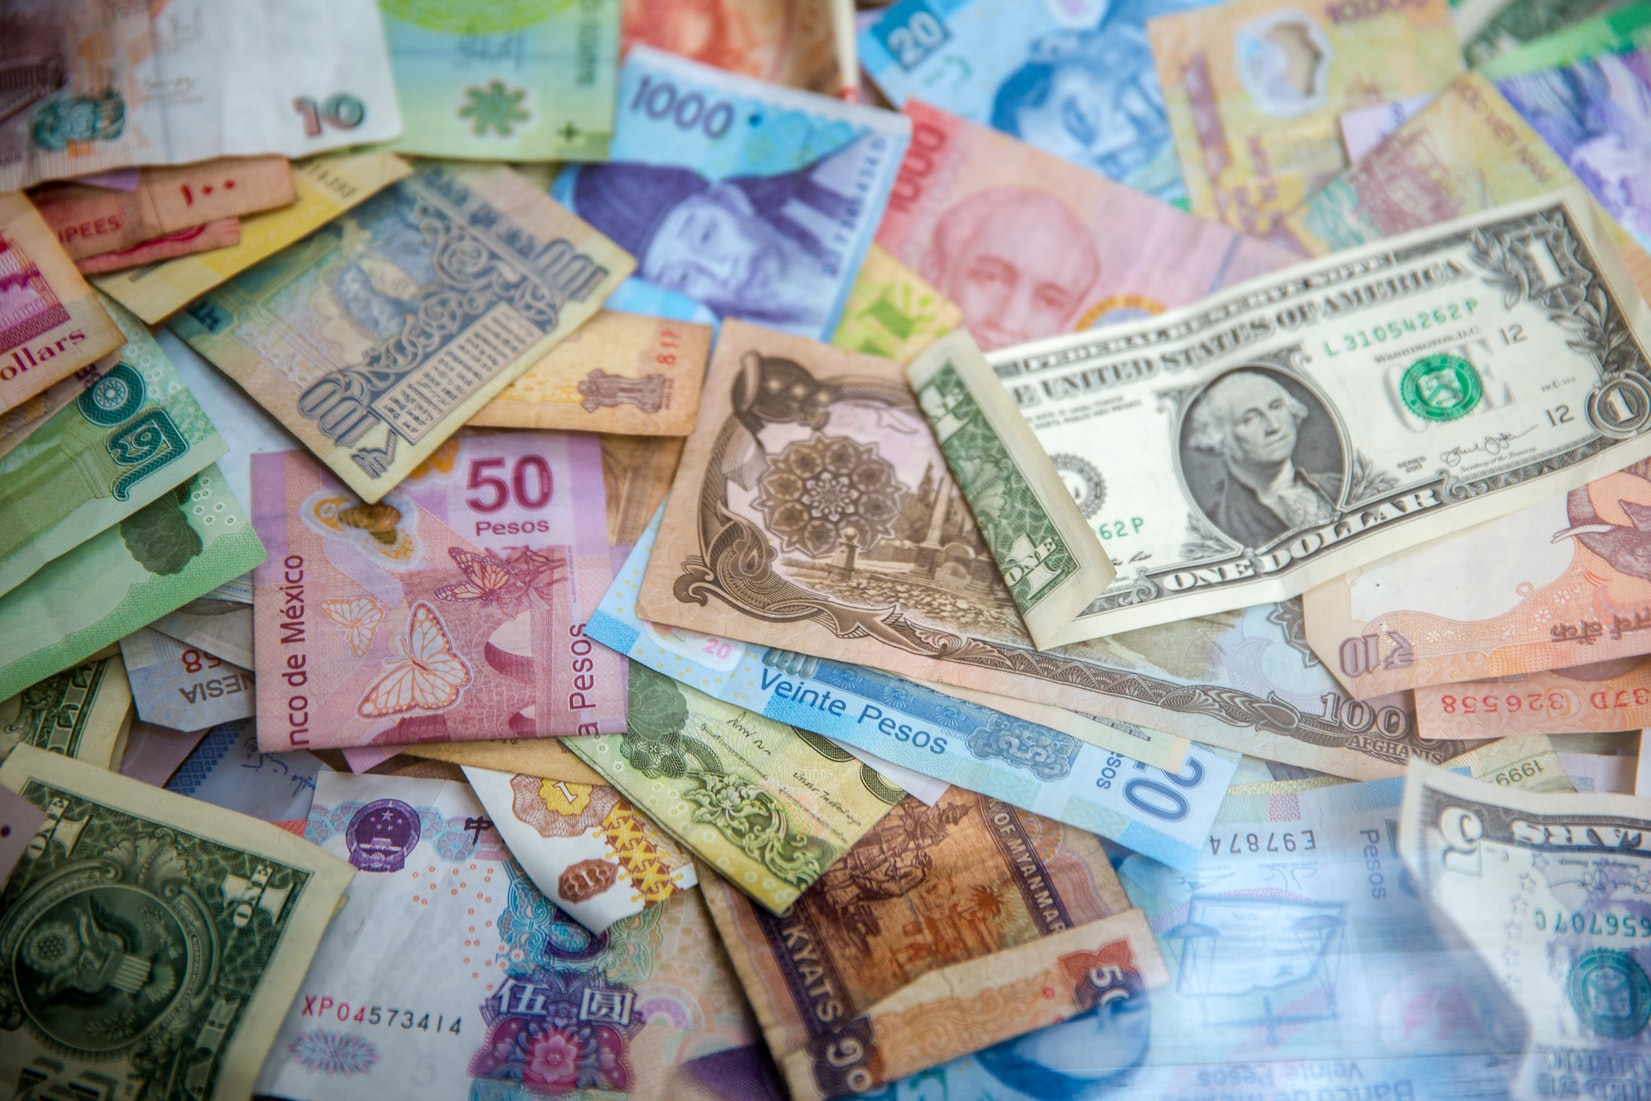
\includegraphics[width=\linewidth]{images/currencies.jpg}			% define cover picture
\end{textblock}


\color{black}

% Institution / titel / subtitel / authors / experts:
%---------------------------------------------------------------------------
\begin{flushleft}

\vspace*{115mm}

\fontsize{24pt}{26pt}\selectfont 
\heading				\\							% Read heading from file leader/title.tex
\vspace{2mm}

\fontsize{14pt}{18pt}\selectfont\vspace{0.3em}
Applied Data Science in an Industrial Banknote Image Recognition Framework			\\				% Insert subheading
\vspace{5mm}


% Abstract (eingeben):
%---------------------------------------------------------------------------


\begin{textblock}{150}(28,225)
\fontsize{10pt}{17pt}\selectfont
\begin{tabbing}
xxxxxxxxxxxxxxx\=xxxxxxxxxxxxxxxxxxxxxxxxxxxxxxxxxxxxxxxxxxxxxxx \kill
Degree course:	\> [BSc Informatik]	\\		% insert name of degree course
Authors:		\> [Sophie Haug]		\\					% insert names
Constituent:	\> [CI Tech Sensors AG]					\\							% insert names
Experts:		\> [Prof. Dr. Macha Kurpicz-Briki]				\\							% insert names
Date:			\> \versiondate					\\							% read from file leader/version.tex
\end{tabbing}

\end{textblock}
\end{flushleft}

\begin{textblock}{150}(28,280)
\noindent 
\color{bfhgrey}\fontsize{9pt}{10pt}\selectfont
Berner Fachhochschule | Haute \'ecole sp\'ecialis\'ee bernoise | Bern University of Applied Sciences
\color{black}\selectfont
\end{textblock}


\end{titlepage}

%
% ===========================================================================
% EOF
%
		% activate for frontpage with picture
% Control of versions :
% -----------------------------------------------

\begin{textblock}{180}(15,150)
\color{black}
\begin{huge}
Versions
\end{huge}
\vspace{10mm}

\fontsize{10pt}{18pt}\selectfont
\begin{tabbing}
xxxxxxxxxxx\=xxxxxxxxxxxxxxx\=xxxxxxxxxxxxxx\=xxxxxxxxxxxxxxxxxxxxxxxxxxxxxxxxxxxxxxxxxxxxxxx \kill
Version	\> Date	\> Status			\> Remarks		\\
0.1	\> 01.08.2013	\> Draft		\> Lorem ipsum dolor sit amet	\\	
0.2	\> 21.08.2013	\> Draft		\> Phasellus scelerisque	\\ 
0.3	\> 02.09.2013	\> Draft		\> Donec eget aliquam urna. Lorem ipsum dolor sit amet	\\ 
1.0	\> 26.01.2014	\> Final		\> Lorem ipsum dolor sit ametPhasellus scelerisque, leo sed iaculis ornare 	\\ 
1.1	\> 31.01.2014	\> Correction	\> Layout changed	\\
1.2	\> 07.02.2014	\> Addition		\> Chapter 1.1 extended	\\
\end{tabbing}

\end{textblock}

\cleardoubleemptypage
\setcounter{page}{1}
\cleardoublepage
\phantomsection 
\addcontentsline{toc}{chapter}{Management Summary}
\chapter*{Abstract}
\label{chap:abstract}

In this project concepts and methods for collecting and preparing data for Currency Adaption are presented, in the context of the company CI Tech Sensors in Burgdorf.
The currency data needed to train and develop algorithms in CI Tech's currency recognition and classification framework should be provided as centralized labelled data sets. These data sets should be generated automatically from the centralized Data Lake. This project proposes a new data container ``NoteSet``, as well as exemplary workflows to achieve this goal.
The implementation was done in Python and using the Jupyter Notebook environment.
\cleardoubleemptypage
%---------------------------------------------------------------------------

% Table of contents
%---------------------------------------------------------------------------
\tableofcontents
\cleardoublepage
%---------------------------------------------------------------------------

% Main part:
%---------------------------------------------------------------------------
\pagenumbering{arabic}

\chapter{Project Goals}
\label{chap:projectgoals}

\section{Initial Position}
\subsection{Background}
The 80/20 rule of Data Science states that most data scientist spend about 20\% of their time on actual data analysis and 80\% of their time finding, cleaning and preparing data. The process of readying data for the training, testing and implementation of an algorithm thus is not only a highly important step in the Data Science Lifecycle, it's maybe the costliest.\par
CI Tech Sensors has over 30 years experience in the field of Banknote Image recognition. One of its core competences is the development of currency adaptation software. Namely the so-called Currency Data File is a software, which is loaded onto the banknote reader, and enables it to identify and classify banknotes for specific currencies, as well as determine their fitness and authenticity. This software is continuously updated and developed by a dedicated team of Currency Adaptation Specialists at CI Tech Sensors, whose work relies on the availability of a huge data pool of Banknote Raw Data. \par
Over the last three years, there has been ground-breaking shift in raw data management: From folder-based data storage on both local and central file drives -  which heavily relied on filenames for identification and was thus prone to ambiguity and duplication of data - towards a centralized data pool, where each file was given a unique ID. At the same time a cloud based Microservice architecture (MOVEm Data Management Toolchain) for the management and maintenance of this data pool was developed.
This development comes with a number of exciting possibilities, some of which to explore is the goal of this project. The focus will be on the collection and preparation of tailored banknote sets.\par

In earlier days, the collection and preparation of banknote data had to be manually done by the Currency Adaptation Specialist. They would have to navigate to the relevant folder, select the relevant files and sort them by denomination, emission, orientation and other criteria, an information taken from a file's annotation. Not only is this process cumbersome and error-prone in itself, it also solely relies on the file annotation, which is made by a human annotator before the actual banknote recording, and thus can contain errors as well. \par
Today it's already possible to group banknote raw data into sets, using a text-based file format called notelist file . Adaptations specialists will manage and create their own notelist files locally according to their specific needs. Notelists contain references to individual file IDs and Note IDs as well as additional annotational information and the file path where files can be found. However this format comes with some problems of its own.\par

\subsection{Overview of the existing CI Tech adaptation toolchain }

In this section a short overview is given over some of the tool in the existing CI Tech adaptation toolchain. This list is by far not exhaustive and only names the tools which are mot relevant to the project at hand
\begin{itemize}
\item \emph{MCM} (MOVE Currency Data Modeller) is a desktop application and the main tool of currency adaptation specialists in their daily work. It is used to develop, test and adapt so called \emph{Currency Data Files}, the software which is loaded onto the banknote reader and enables it to recognize and classify banknotes. MCM is a software monolith that has grown and extended its functionality over decades, but it doesn't lend itself very easily to modularization. MCM is also the interface to the entire algorithmic framework. Recordings of banknotes can be loaded from the filesystem as .NIF files (binary files) or .nl (XML Format) files. The latter also allows loading notes from the central Data Pool via MFX instead of the local file system.

\item \emph{MFX} (MOVE File Index) is a web based microservice that allows the lookup of files from the central Data Pool. Namely, it allows to retrieve the storage path in the pool for a given File ID. Using this service, MCM can load files by File ID instead of a file path.

\item \emph{MDS} (MOVE Data Service) is a web based microservice that allows the lookup of note and image data. It allows to query the most relevant note data found in the (binary) .NIF files as well as images via REST api. A future vision which is in ongoing development is that entire sets of notes could be loaded into MCM via this REST interface instead of parsing large amounts of binary data. 


\end{itemize}
\subsection{Stakeholders}
\begin{itemize}
\item The Head of Application Software will supervise the project and provide technical advice
\item The Head of Currency Adaptation will provide additional support from the perspective of Currency Adaptation specialists.
\item The Currency Adaptation team will be the primary user group
\end{itemize}

\section{Project Goals}
\label{sec:goals}


\subsection{Accurate, consistent and complete reference data sets}
The goal is to have accurate and consistent data sets, which are generated and persisted in a way that makes use of the Microservice based MOVEm Data Management Toolchain. Namely these test sets should fulfil the following criteria:

\begin{itemize}
\item Accuracy: Data in test sets has been checked for correct labeling and or given a label in case it was missing.
\item Consistency: Different adaptations for the same currency should use the same data sets. 
\item Completeness: In the generation of reference note data sets, all data in the pool should be considered.

\end{itemize}




\subsection{Mechanism for subclassifying Data Sets according to context-dependent criteria}

It should be possible to generate data sets according to user specific criteria like: "All EUR notes that were classified as fake", "All USD notes for which tape was detected". 
A process should be installed which allows specialist users to generate such datasets from queries. These datasets will have to fulfil the same criteria as the reference data sets.

\subsection{Automated process for generating and maintaining Reference Note Data Sets}

A process has to be defined for generating Reference Data Sets automatically as well as updating and expanding them when new data is added to the Data Pool. A process has to be defined for generating Reference Data Sets automatically as well as updating them when new data is added to the Data Pool. Part of this process is also the management of Reference Data Sets in a Version Control System. 

\subsection{Technical Analysis of the existing Toolchain}

To achieve the previously listed goals, the introduction of a new data container will be necessary to make the existing toolchain compatible with this new paradigm. While this shift can only happen over a longer period, it would be very undesirable to have a new data container or format which will only be deployable for a part of the toolchain. The goal is therefore to have an assessment on the feasibility of implementing the new data container into the existing toolchain. 


\subsection{Introduction of Data Science Workflows in the company}
Another less technical goal, is to familiarize users with certain Data Science workflows. This entails showing by presenting this project how the existing microservice can be used to gain knowledge about note data and generate data sets, as well as familiarize expert users (who might want to use similar workflows to generate their own data sets) with the Jupyter Notebook framework.
\chapter{Instructions}
\label{chap:instructions}

The following table shows some of the most important packages\index{packages} used in the \LaTeX{} template.

\begin{table}[H]
	\centering
		\begin{tabular}{p{0.13\textwidth} p{0.75\textwidth}} \toprule
			\textbf{Package} & \textbf{Function} \\ \midrule
			\texttt{cmbright}\index{cmbright} & sans serif font "Computer Modern Bright", which supports text encodings\index{text encodings} OT1, T1 and TS1, as well as the mathematical signs and AMS symbols \\ \midrule
			\texttt{ae} & provides better resolution fonts in PDF files \\ \midrule
			\texttt{fancyhdr}\index{fancyhdr} & easy adjustment of head- and foot lines \\ \midrule
			\texttt{graphicx}\index{graphicx} & integration of graphics in \LaTeX{} documents \\ \midrule
			\texttt{booktabs}\index{booktabs} & better presentation of tables \\ \midrule
			\texttt{textpos}\index{textpos} & simplified and absolute positioning of boxes on the page \\ \midrule
			\texttt{hyperref}\index{hyperref} & package to complie links into PDF files \\ \midrule
			\texttt{geometry}\index{geometry} & simplified and improved adaptation of the standard type area \\ \midrule
			\texttt{makeidx}\index{makeidx} & simple Index compilation (see section \ref{sec:instructions_index}) \\ \midrule
			\texttt{glossaries}\index{glossaries} & compilation of glossaries (see section \ref{sec:instructions_glossay}) \\ \bottomrule
		\end{tabular}
	\caption{Packages}
	\label{tab:packages}
\end{table}


\section{Subject Indices}
\label{sec:instructions_index}

\LaTeX{} is not able to create an \gls{Index}\index{Index} in the basic configuration. This can be created in \LaTeX{} with the \texttt{makeidx} package and the \texttt{makeindex}\index{makeindex} program. The following page contains a detailed explanation of how the package works, and its application:

\begin{center}
	\url{http://en.wikibooks.org/wiki/LaTeX/Indexing}
\end{center}

Roughly summarized the following points are needed for an index:

\begin{itemize}
	\item Embed the package \texttt{makeidx}.
	\item Initialize the compilation with the command \texttt{\textbackslash makeindex}.
	\item Continuously initializing words in the text with the command \texttt{\textbackslash index\{\}}.
	\item During the first passage of the document's compilation, the directory is created and definitions marked with \texttt{\textbackslash index\{\}} are stored in the \texttt{.idx} file.
	\item During the second passage the \texttt{.idx} file is sorted, formatted and stored as \texttt{.ind} file whereas \LaTeX{} then inserts the \texttt{.ind} file into the document.
\end{itemize}

\section{Glossay}
\label{sec:instructions_glossay}

A glossary\index{glossary} can also be created in \LaTeX{} with the \texttt{makeindex} program and the \texttt{glossaries} package. The following list shows the procedure to generate a glossary:

\begin{itemize}
	\item Integration of the package \texttt{glossaries}.
	\item If necessary, a personal database may be created including glossary entries. This template works with such a database, which is stored in the \texttt{database}folder. Entries from the database are only written in the directory if the word in the text is actually stated.
	\item With the \texttt{\textbackslash makeglossaries} command a new compilation is initialized.
	\item New entries can be created with the command \\ \texttt{\textbackslash newglossaryentry\{<SHORTCUT>\}\{name=\{<NAME>\},description=\{<DESCRIPTION>\}\}}.
	\item In the text continuously referencing words with the command \texttt{\textbackslash gls\{<SHORTCUT>\}}.
	\item Similar to the compilation of the index, the directory is only embedded into the document  during the second passage.
\end{itemize}

In order to work accurately, the glossary must be compiled with \texttt{makeindex} after post-editing the document. For this the following code in the command line is to be executed:

\begin{center}
	\texttt{makeindex -s template.ist -t template.glg -o template.gls template.glo}
\end{center}

With most \LaTeX editors, this can be stated as a post-processing step. The following explanation is for the TeXnicCenter program. Under the menu "Build" > "Define Output Profile..." (short: alt + F7) in the "Postprocessor" register, the window shown in Figure \ref{fig:postprocessing} can be found. Then it is necessary to insert a new entry, when an application as well as an argument must be specified. The application can be found in the MiKTeX installation (\texttt{..\textbackslash MiKTeX X.X\textbackslash miktex\textbackslash bin\textbackslash makeindex.exe}). As an argument, the following line must be entered:

\begin{center}
	\texttt{-s \string"\%tm.ist\string" -t \string"\%tm.glg\string" -o \string"\%tm.gls\string" \string"\%tm.glo\string" }
\end{center}

\begin{figure}[H]
	\centering
		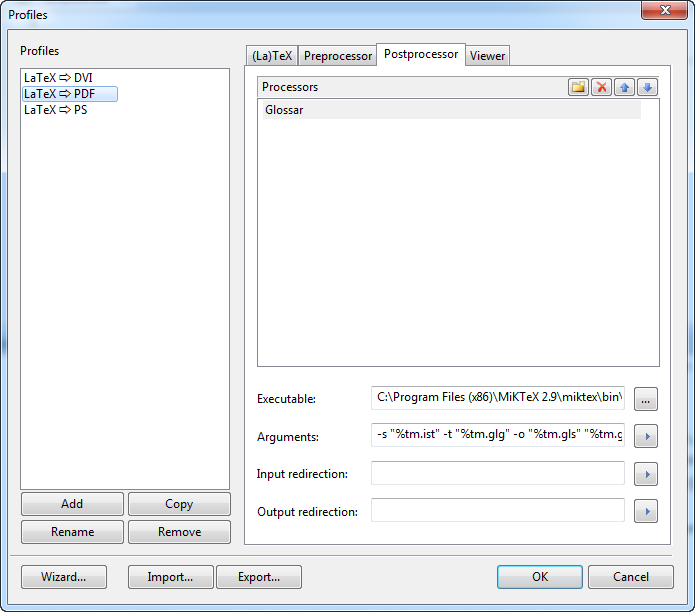
\includegraphics[scale=0.6]{images/profiles_glossar.png}
	\caption{Post-processing}
	\label{fig:postprocessing}
\end{figure}


\section{Bibliography}
\label{sec:instructions_bibliography}

To compile a bibliography\index{bibliography} one must resort to \gls{BibTeX}. The folder \texttt{database} includes a \texttt{.bib} file with various database entries. How the entries are to be compiled, can be taken from various sources of the Internet or books. The entries in the database will only be written to the directory of the document when the source is actually cited in the text.

Under the following addresses further explanations are found in order to compile the database and its use:

\begin{itemize}
	\item \url{http://en.wikipedia.org/wiki/BibTeX}
	\item \url{http://www.bibtex.org/}
\end{itemize}



\chapter{Test of type area}
\label{chap:typeareatest}

Far far away, behind the word mountains, far from the countries Vokalia and Consonantia, there live the blind texts. Separated they live in Bookmarksgrove right at the coast of the Semantics, a large language ocean. A small river named Duden flows by their place and supplies it with the necessary regelialia. It is a paradisematic country, in which roasted parts of sentences fly into your mouth. Even the all-powerful Pointing has no control about the blind texts it is an almost unorthographic life One day however a small line of blind text by the name of Lorem Ipsum decided to leave for the far World of Grammar. 

\section{The Big Oxmox}
\label{sec:typeareatest_ombox}

The Big Oxmox advised her not to do so, because there were thousands of bad Commas, wild Question Marks and devious Semikoli, but the Little Blind Text didn’t listen. She packed her seven versalia, put her initial into the belt and made herself on the way. When she reached the first hills of the Italic Mountains, she had a last view back on the skyline of her hometown Bookmarksgrove, the headline of Alphabet Village and the subline of her own road, the Line Lane. Pityful a rethoric question ran over her cheek, then she continued her way. On her way she met a copy.

\begin{equation}
	\mathcal{N}(x \mid \mathbold{\mu}, \mathbold{\Sigma}) = \frac{1}{(2\pi)^{D/2}} \frac{1}{|\mathbold{\Sigma}|^{(1/2)}} \exp \left( -\frac{1}{2}(x-\mathbold{\mu})^{T}\mathbold{\Sigma}^{-1}(x-\mathbold{\mu}) \right)
\end{equation}

The copy warned the Little Blind Text, that where it came from it would have been rewritten a thousand times and everything that was left from its origin would be the word "and" and the Little Blind Text should turn around and return to its own, safe country. But nothing the copy said could convince her and so it didn’t take long until a few insidious Copy Writers ambushed her, made her drunk with Longe and Parole and dragged her into their agency, where they abused her for their projects again and again. And if she hasn’t been rewritten, then they are still using her.

\section{Type dummy text}
\label{sec:typeareatest_typedummytext}

This is a typo dummy text. On it you can see if all the letters there are and how they look. Sometimes one uses words like Hamburgefonts, Rafgenduks or Handgloves to test fonts. Sometimes phrases that contain all letters of the alphabet - one calls these sets "pangrams".

Well known is this: The quick brown fox jumps over the lazy old dog. Often in type dummy texts also foreign-language sentence parts are installed (AVAIL\textsuperscript{\texttrademark} and Wefox\textsuperscript{\textregistered} are testing aussi la Kerning) to test the effect in other languages. In Latin, for example, almost every font looks good.

\subsection{Demonstrandum}
\label{subsec:satzspiegeltest_typoblindtext_demonstrandum}

Quod erat demonstrandum. Seit 1975 fehlen in den meisten Testtexten die Zahlen, weswegen nach TypoGb. 204 \S ab dem Jahr 2034 Zahlen in 86 der Texte zur Pflicht werden. Nichteinhaltung wird mit bis zu 245 \texteuro oder 368\$ bestraft. Genauso wichtig in sind mittlerweile auch \^A\c{c}c\`e\~nt\"e, die in neueren Schriften aber fast immer enthalten sind. Ein wichtiges aber schwierig zu integrierendes Feld sind OpenType-Funktionalit\"aten. Je nach Software und Voreinstellungen k\"onnen eingebaute Kapit\"alchen, Kerning oder Ligaturen (sehr pfiffig) nicht richtig dargestellt werden.

\subsubsection{Subsubsection}

This is a typo dummy text. On it you can see if all the letters there are and how they look. Sometimes one uses words like Hamburgefonts, Rafgenduks or Handgloves to test fonts. Sometimes phrases that contain all letters of the alphabet - one calls these sets "pangrams". 

\subsubsection{Subsubsection}

Well known is this: The quick brown fox jumps over the lazy old dog. Often in type dummy texts also foreign-language sentence parts are installed (AVAIL\textsuperscript{\texttrademark} and Wefox\textsuperscript{\textregistered} are testing aussi la Kerning) to test the effect in other languages. In Latin, for example, almost every font looks good. Quod erat demonstrandum.

\section{Webstandards}
\label{sec:satzspiegeltest_webstandards}

Everywhere the same old story. The layout is complete, the text is slow in coming. This layout is now not naked in space and small and empty occurs, I help out: the dummy text. Created exactly for this purpose, always in the shadow of my big brother "Lorem Ipsum", I look forward every time you read a few lines. Because esse est percipi - being is to be perceived.

And now because you already have the goodness to accompany me a few more sentences long, I would like to take this opportunity to serve you not only as a stopgap, but to point out something that is going to be perceived as deserved: Web viz. See Web standards are the rules that build on the websites. So there are rules for HTML, CSS, JavaScript or XML, words that you might have heard of your developers. These standards ensure that all parties the maximum benefit from a website.

\begin{figure}[H]
	\centering
		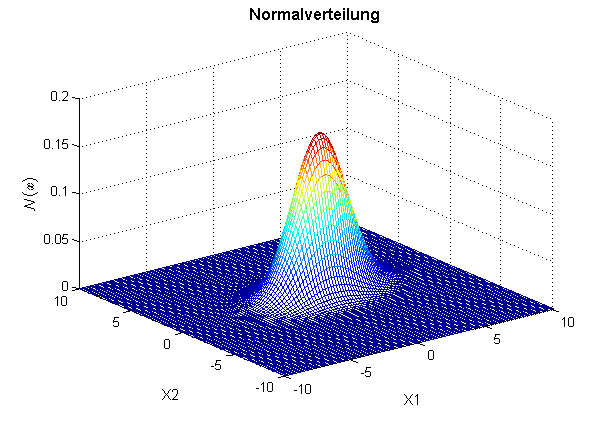
\includegraphics[scale=0.7]{images/multivariate_gauss.png}
	\caption{Normal distribution}
	\label{fig:normal_distribution}
\end{figure}

In contrast to previous websites we no longer need, for example, two different sites for the program Internet Explorer and another browser. It extends a page that - properly applied - both works on different browsers on the net, but just as good for printing or display on a cell phone is. Mind: A site for all formats. What a relief. Standards save time provide for the development costs and ensure that web pages can be easier to maintain later. Of course, only if everyone adheres to these standards.

\chapter{Conclusion / Results}
\label{chap:conclusions}

But I must explain to you how all this mistaken idea of denouncing pleasure and praising pain was born and I will give you a complete account of the system, and expound the actual teachings of the great explorer of the truth, the master-builder of human happiness. No one rejects, dislikes, or avoids pleasure itself, because it is pleasure, but because those who do not know how to pursue pleasure rationally encounter consequences that are extremely painful. Nor again is there anyone who loves or pursues or desires to obtain pain of itself, because it is pain, but because occasionally circumstances occur in which toil and pain can procure him some great pleasure. To take a trivial example, which of us ever undertakes laborious physical exercise, except to obtain some advantage from it? But who has any right to find fault with a man who chooses to enjoy a pleasure that has no annoying consequences, or one who avoids a pain that produces no resultant pleasure? On the other hand, we denounce with righteous indignation and dislike men who are so beguiled and demoralized by the charms of pleasure of the moment, so blinded by desire, that they cannot foresee the pain and trouble that are bound to ensue; and equal blame belongs to those who fail in their duty through weakness of will, which is the same as saying through shrinking from toil and pain. These cases are perfectly simple and easy to distinguish. In a free hour, when our power of choice is untrammelled and when nothing prevents our being able to do what we like best, every pleasure is to be welcomed and every pain avoided. But in certain circumstances and owing to the claims of duty or the obligations of business it will frequently occur that pleasures have to be repudiated and annoyances accepted. The wise man therefore always holds in these matters to this principle of selection: he rejects pleasures to secure other greater pleasures, or else he endures pains to avoid worse pains.

\newpage

But I must explain to you how all this mistaken idea of denouncing pleasure and praising pain was born and I will give you a complete account of the system, and expound the actual teachings of the great explorer of the truth, the master-builder of human happiness. No one rejects, dislikes, or avoids pleasure itself, because it is pleasure, but because those who do not know how to pursue pleasure rationally encounter consequences that are extremely painful. Nor again is there anyone who loves or pursues or desires to obtain pain of itself, because it is pain, but because occasionally circumstances occur in which toil and pain can procure him some great pleasure. To take a trivial example, which of us ever undertakes laborious physical exercise, except to obtain some advantage from it? But who has any right to find fault with a man who chooses to enjoy a pleasure that has no annoying consequences, or one who avoids a pain that produces no resultant pleasure? On the other hand, we denounce with righteous indignation and dislike men who are so beguiled and demoralized by the charms of pleasure of the moment, so blinded by desire, that they cannot foresee the pain and trouble that are bound to ensue; and equal blame belongs to those who fail in their duty through weakness of will, which is the same as saying through shrinking from toil and pain. These cases are perfectly simple and easy to distinguish. In a free hour, when our power of choice is untrammelled and when nothing prevents our being able to do what we like best, every pleasure is to be welcomed and every pain avoided. But in certain circumstances and owing to the claims of duty or the obligations of business it will frequently occur that pleasures have to be repudiated and annoyances accepted. The wise man therefore always holds in these matters to this principle of selection: he rejects pleasures to secure other greater pleasures, or else he endures pains to avoid worse pains.

%---------------------------------------------------------------------------

% Declaration of Authorship
%---------------------------------------------------------------------------
\cleardoublepage
\phantomsection 
\addcontentsline{toc}{chapter}{Declaration of authorship}
\chapter*{Declaration of primary authorship}
\label{chap:declaration_authorship}

\vspace*{10mm} 

I / We hereby confirm that I / we have written this thesis independently and without using other sources and resources than those specified in the bibliography. All text passages which were not written by me are marked as quotations and provided with the exact indication of its origin. 

\vspace{15mm}

\begin{tabbing}
xxxxxxxxxxxxxxxxxxxxxxxxxxxxxx\=xxxxxxxxxxxxxxxxxxxxxxxxxxxxxx\=xxxxxxxxxxxxxxxxxxxxxxxxxxxxxx\kill
Place, Date:		\> [Biel/Burgdorf], \versiondate \\ \\ 
Last Name/s, First Name/s:	\> [Test Peter] 	\> [M\"uster R\"os\"a] \\ \\ \\ \\ 
Signature/s:	\> ......................................\> ...................................... \\
\end{tabbing}

%---------------------------------------------------------------------------

% Glossary
%---------------------------------------------------------------------------
\cleardoublepage
\phantomsection 
\addcontentsline{toc}{chapter}{Glossay}
%\renewcommand{\glossaryname}{Glossay}
\printglossary
%---------------------------------------------------------------------------

% Bibliography
%---------------------------------------------------------------------------
\cleardoublepage
\phantomsection 
\addcontentsline{toc}{chapter}{Bibliography}
\bibliographystyle{IEEEtranS}
\bibliography{database/bibliography}{}
%---------------------------------------------------------------------------

% Listings
%---------------------------------------------------------------------------
\cleardoublepage
\phantomsection 
\addcontentsline{toc}{chapter}{List of figures}
\listoffigures
\cleardoublepage
\phantomsection 
\addcontentsline{toc}{chapter}{List fo tables}
\listoftables
%---------------------------------------------------------------------------

% Index
%---------------------------------------------------------------------------
\cleardoublepage
\phantomsection 
\addcontentsline{toc}{chapter}{Index}
\printindex
%---------------------------------------------------------------------------

% Attachment:
%---------------------------------------------------------------------------
\appendix
\settocdepth{section}
\chapter*{APPENDICES}
\addcontentsline{toc}{chapter}{APPENDICES}

\begingroup\let\clearpage\relax
\chapter{The pynoteset library}
\label{chap:appendix_pns}
\endgroup

The pynoteset library was developed within the scope of this project. Its purpose is to generate and handle the newly introduced NoteSet data container. This small library can theoretically be deployed in the entire Python toolchain of application software at CI Tech. An analogous implementation in C\# for the .NET toolchain is still pending

\section{The NoteSet class}
This is the base class representing a noteset object. A NoteSet represents a set of Note IDs. It can optionally contain an annotation property, which is of type NoteSetAnnotation.
\subsection{from\_note\_id\_list(note\_id\_list)}
\subsubsection{Description}
Generates a NoteSet object from a list of Note IDs
\subsubsection{Parameters}
\begin{description}
\item [note\_id\_list] A list of strings representing Note IDs.

\end{description}

\subsection{from\_note\_id\_list\_and\_annotation(note\_id\_list, annotation)}
\subsubsection{Description}
Generates a NoteSet object from a list of Note IDs and a NoteSetAnnotation object.
\subsubsection{Parameters}
\begin{description}
\item [note\_id\_list] A list of strings representing Note IDs.
\item [annotation] NoteSetAnnotation
\end{description}


\subsection{from\_notelistfile(nl\_file)}
\subsubsection{Description}
Generate a NoteSet object from a Notelistfile object, i.e. convert a Notelistfile into a NoteSet.
\subsubsection{Parameters}
\begin{description}
\item [nl\_file] Notelistfile 
\end{description}

\subsection{diff(noteset\_1, noteset\_2)}
\subsubsection{Description}
Find the difference of two NoteSets. Return two notesets:
\begin{itemize}
	\item NoteSet of all elements contained in noteset\_1 but not noteset\_2
	\item NoteSet of all elements contained in noteset\_2 but not noteset\_1
\end{itemize}
\subsubsection{Parameters}
\begin{description}
\item [noteset\_1] NoteSet
\item [noteset\_2] NoteSet
\end{description} 

\subsection{merge(noteset\_1, noteset\_2)}
\subsubsection{Description}
Merge two NoteSets into a new NoteSet
\subsubsection{Parameters}
\begin{description}
\item [noteset\_1] NoteSet
\item [noteset\_2] NoteSet
\end{description} 

\subsection{export\_to\_ns\_file(filepath)}
\subsubsection{Description}
Save a NoteSet as ASCII file
\subsubsection{Parameters}
\begin{description}
\item [filepath] string or path-like object
\end{description}
\chapter{Additional Appendix}
\label{chap:appendix_B}

\section{Test 1}
To an English person, it will seem like simplified English, as a skeptical Cambridge friend of mine told me what Occidental is. The European languages are members of the same family. Their separate existence is a myth. For science, music, sport, etc, Europe uses the same vocabulary. The languages only differ in their grammar, their pronunciation and their most common words. Everyone realizes why a new common language would be desirable: one could refuse to pay expensive translators. To achieve this, it would be necessary to have uniform grammar, pronunciation and more common words. If several languages coalesce, the grammar of the resulting language is more simple and regular than that of the individual languages. The new common language will be more simple and regular than the existing European languages. 

\subsection{Environment}
It will be as simple as Occidental; in fact, it will be Occidental. To an English person, it will seem like simplified English, as a skeptical Cambridge friend of mine told me what Occidental is. The European languages are members of the same family. Their separate existence is a myth. For science, music, sport, etc, Europe uses the same vocabulary. The languages only differ in their grammar, their pronunciation and their most common words. Everyone realizes why a new common language would be desirable: one could refuse to pay expensive translators. To achieve this, it would be necessary to have uniform grammar, pronunciation and more common words.
\chapter{Content of CD-ROM}
\label{chap:appendix_CDROM}

Content of the enclosed CD-ROM, directory tree, etc.
%---------------------------------------------------------------------------

%---------------------------------------------------------------------------
\end{document}

